\documentclass[paper=a4, fontsize=11pt]{scrartcl} % A4 paper and 11pt font size

\usepackage[T1]{fontenc} % Use 8-bit encoding that has 256 glyphs
\usepackage{utopia} % Use the Adobe Utopia font for the document - comment this line to return to the LaTeX default
\usepackage[english]{babel} % English language/hyphenation
\usepackage{amsmath,amsfonts,amsthm} % Math packages
\usepackage{sectsty} % Allows customizing section commands
\allsectionsfont{\centering \normalfont\scshape} % Make all sections centered, the default font and small caps
\usepackage{fancyhdr} % Custom headers and footers
\pagestyle{fancyplain} % Makes all pages in the document conform to the custom headers and footers
\fancyhead{} % No page header - if you want one, create it in the same way as the footers below
\fancyfoot[L]{} % Empty left footer
\fancyfoot[C]{} % Empty center footer
\fancyfoot[R]{\thepage} % Page numbering for right footer
\renewcommand{\headrulewidth}{0pt} % Remove header underlines
\renewcommand{\footrulewidth}{0pt} % Remove footer underlines
\setlength{\headheight}{13.6pt} % Customize the height of the header
\numberwithin{equation}{section} % Number equations within sections (i.e. 1.1, 1.2, 2.1, 2.2 instead of 1, 2, 3, 4)
\numberwithin{figure}{section} % Number figures within sections (i.e. 1.1, 1.2, 2.1, 2.2 instead of 1, 2, 3, 4)
\numberwithin{table}{section} % Number tables within sections (i.e. 1.1, 1.2, 2.1, 2.2 instead of 1, 2, 3, 4)
\usepackage{graphicx}

\setlength\parindent{0pt} % Removes all indentation from paragraphs - comment this line for an assignment with lots of text
% \addtolength{\oddsidemargin}{-.15in}
% \addtolength{\evensidemargin}{-0.15in}
% \addtolength{\textwidth}{-0.5in}
\addtolength{\topmargin}{-0.5in}
\addtolength{\textheight}{1.2in}
\addtolength{\evensidemargin}{-.5in}
\addtolength{\oddsidemargin}{-.5in}
\addtolength{\textwidth}{.5in}


\newcommand{\horrule}[1]{\rule{\linewidth}{#1}} % Create horizontal rule command with 1 argument of height

\title{	
\normalfont \normalsize 
% \textsc{university, school or department name} \\ [25pt] % Your university, school and/or department name(s)
\horrule{0.5pt} \\[0.4cm] % Thin top horizontal rule
\huge{10-605 Assignment 5: Stochastic Gradient Descent} \\ % The assignment title
\horrule{2pt} \\[0.5cm] % Thick bottom horizontal rule
}

\author{Namit Katariya (andrew id: nkatariy)} % Your name
\date{\normalsize\today} % Today's date or a custom date

\begin{document}

\maketitle 
\vspace*{-0.65in}
\section*{\textbf{Question 0}}

\begin{itemize}
\item \underline{Output of "make demo" with dictionary size 10000 and $\mu=$0.1 (cumulative log probability printed)}:
\begin{verbatim}
[pt,tr,hu,es,ru,pl,ca,nl,sl,fr,ga,de,hr,el]	[es,fr]	   -2.5163927479098613
[es,ru,ca,fr,de,el]	                        [de,fr,pt]	-5.230361667820243
[pt,es,ru,pl,fr,de]	                        [de,pl]	   -4.52829260056261
[pt,es,ru,fr,de]	                           [fr,pt]	   -3.119880323675378
[es,pl,fr,de]	                              [es,fr]    -3.6469902180384097
[pl,ca,de]	                                 [pl]	      -6.194962572700562
[pt,de]	                                    [fr]	      -5.204173354282212
[pt,es,pl,fr,de]	                           [fr,pt]	   -4.178269526803922
[es,ru,de]	                                 [fr,pl]	   -5.451279489139332
[fr,de]	                                    []	        -4.61184834723814
[nl]	                                       [de,fr]	   -5.268614630149776
[fr,ga]	                                    [pl]	      -5.176682704814612
[hu]                                      	 []	        -5.448188469812148
[fr]	                                       [de,fr,pl] -4.00770730247661
[fr,de]	                                    []	        -5.751580796391452
[pt,es,pl,ca,nl,fr]	                        [fr,nl,pl]	-5.9053061640367215
[el]	                                       [fr]	      -6.414965515545923
[de]	                                       [fr]	      -3.656166537983577
[fr]                                     	  []	        -6.001685320724161
[pt,fr]	                                    [fr]	      -5.740815356797156
[pl]                                       	[pl]	      -4.1147689641279035
[ru,pl,de]	                                 []	        -5.770545344041741
[fr]	                                       [fr,pl]	   -6.208966918246572
[pt,fr]	                                    [fr]	      -5.5445391905239445
[sl,fr,de]	                                 []	        -4.987012844617406
[nl]                                       	[fr]	      -4.694053267689198
[ru,pl]                                   	 [de,fr]	   -4.248049647959551
[pt,tr,es,ru,pl,ca,nl,fr,de,el]           	 [pl]	      -5.815795450781371
[pt,es,ru,nl,fr,de]	                        []	        -5.323053944743495

Average acuracy = 77.83251231527095
\end{verbatim}

\item
\begin{tabular}{|l | c|}
\hline
\textbf{Dataset} & \textbf{Average Accuracy (DSIZE=10000, $\mu$=0.1)} \\
\hline
abstract.tiny & 77.83 \\
abstract.small & 80.74 \\
abstract.full & 80.88 \\

\hline
\end{tabular}
\end{itemize}

\section*{\textbf{Question 1}}
\underline{Log likelihood output for small with dictionary size 10000 and $\mu=$0.1}:
\begin{verbatim}
Iteration 1 completed. Log likelihood = -225451.68894086138
Iteration 2 completed. Log likelihood = -119668.6646817663
Iteration 3 completed. Log likelihood = -81665.64888866481
Iteration 4 completed. Log likelihood = -75234.34805401159
Iteration 5 completed. Log likelihood = -79339.44604580262
Iteration 6 completed. Log likelihood = -71771.53539579625
Iteration 7 completed. Log likelihood = -70580.47798692425
Iteration 8 completed. Log likelihood = -71707.37029522772
Iteration 9 completed. Log likelihood = -72867.84522933248
Iteration 10 completed. Log likelihood = -71147.94864523961
Iteration 11 completed. Log likelihood = -69078.08076103363
Iteration 12 completed. Log likelihood = -70697.39971563085
Iteration 13 completed. Log likelihood = -68465.81645070107
Iteration 14 completed. Log likelihood = -70064.93403673773
Iteration 15 completed. Log likelihood = -69939.81033543663
Iteration 16 completed. Log likelihood = -70439.52801302719
Iteration 17 completed. Log likelihood = -69886.82131295884
Iteration 18 completed. Log likelihood = -69350.2999505788
Iteration 19 completed. Log likelihood = -68635.54210052846
Iteration 20 completed. Log likelihood = -68808.25621767242
\end{verbatim}

\section*{\textbf{Question 2}}
Dictionary size 10000 \\
\begin{tabular}{ | c |c | c | c | c | c | c | c | c | c | c | c |}
\hline
$\mu$ & 0 & 1e-6 & 1e-5 & 1e-4 & 1e-3 & 0.01 & 0.1 & 0.2 & 0.3 & 0.5 & 1 \\
\hline
Avg. accuracy & 80.68 & 80.71 & 81.13 & 80.75 & 80.68 & 80.79 & \textbf{81.17} & 81.10 & 81.08 & 80.76 & 80.73 \\
\hline
\end{tabular}

\begin{center}
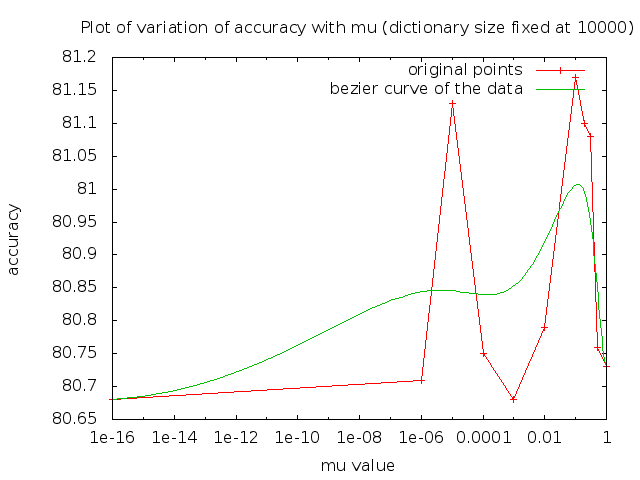
\includegraphics[scale=0.7]{mu-vs-accuracy.png}
\end{center}

\section*{\textbf{Question 3}}
$\mu=$ 0.1 \\
\begin{tabular}{ | c | c | c | c | c | c | c |}
\hline
Dictionary size & 10 & 100 & 1000 & 1e4 & 1e5 & 1e6 \\
\hline
Avg. accuracy & 70.11 & 76.86 &	80.45 & 80.88 & 81.02 & 80.55 \\
\hline
\end{tabular}

\begin{center}
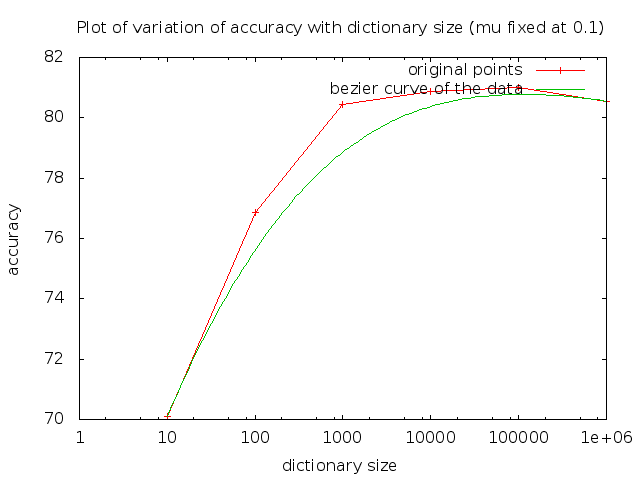
\includegraphics[scale=0.7]{dictionarysize-vs-accuracy.png}
\end{center}

\section*{\textbf{Question 4}}
This is what I did : Along with the messages I was printing earlier, I also printed out messages for labels "NOT"+label. So for instance, if an example does not have "ca" in it true labels, the same messages will be printed out with label="NOTca". The idea is that the entire document is now effective treated as 14 documents for the binary (multi-label as before with number of labels = 2) Naive Bayes classification task for each of the 14 labels. I appropriately changed the log probability calculations and outputted average accuracy as in the current assignment.  \\

\begin{tabular}{| c | c | c |}
\hline
\textbf{Dataset} & \textbf{NaiveBayes} & \textbf{SGD} \\
\hline
Tiny & 40.39	 & 77.83 \\
\hline
Small &	80.26 & 80.74 \\
\hline
Full	 & 82.41 & 80.88 \\
\hline
\end{tabular}

\pagebreak

\section*{\textbf{Bonus Question}}
\begin{itemize} 
\item It was interesting to see the log likelihood values. They decrease upto a point but then increase, then again go down and so on. It's nice that it matches with the understanding that once you reach a trough, based on the learning rate you may sometimes overshoot and even decrease your objective (in a maximization problem)
\item The average accuracy of Naive Bayes on the tiny dataset is around 40\%. Since we are effectively learning 14 binary classifiers, we would expect the average to be at least better than 50\% i.e the average accuracy of a purely random classifier. However, that is not the case. So this was something unexpected
\item I don't know what the results would be with scaling the features to make them have similar ranges but I read online that that is important in logistic type classifiers. So I'm interested in finding out how those results would look. I did ask this question on the google group but no one responded. Also since I did not have much time, I did not try implementing what I myself suggested in the post.
\end{itemize}

\end{document}